%%%%%%%%%%%%%%%%%%%%
% Introduction chapter

%%%%%%%%%%%%%%%%%%%%%%%%%%%%%%%%%%%%%%%%
%%%%%%%%%%%%%%%%%%%%%%%%%%%%%%%%%%%%%%%%
\section{An overview of meiotic recombination}
%%%%%%%%%%%%%%%%%%%%%%%%%%%%%%%%%%%%%%%%
%%%%%%%%%%%%%%%%%%%%%%%%%%%%%%%%%%%%%%%%

Meiosis occurs in all sexually reproducing organisms, and is essential to the generation of gametes.
Recombination plays a key role in this process, facilitating the pairing and alignment of chromosomes, while the exchange of genetic material has important implications in inheritance, natural selection, and evolution.

\afterpage{
\begin{figure}[P]
    \begin{center}
    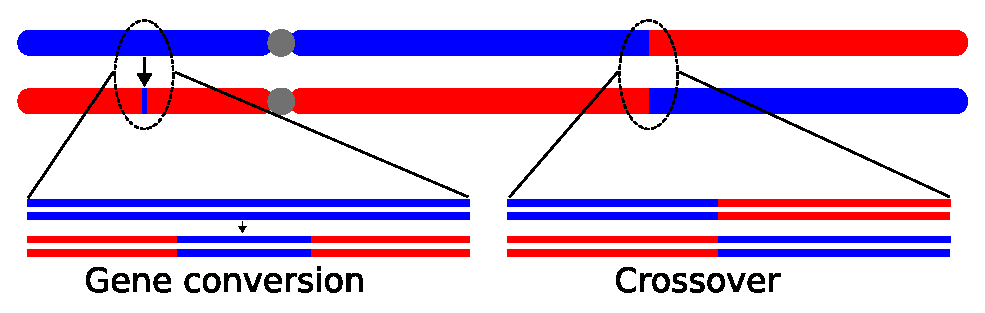
\includegraphics[width=\textwidth]{introduction/figs/outcome_CO-GC}
    \end{center}
    \vspace{-10pt}
    \captionTitle{\textbf{Recombination produces crossover and gene conversion.}}{ 
        Recombination is initiated by DNA double strand breaks that resolve into one of two possible outcomes.
        Crossover (shown at right) is the large-scale, reciprocal exchange of genetic material between two chromosomes around the break point.
        Gene conversion (or non-crossover, shown at left) is the one-way transfer of small amounts of DNA from one chromosome to the other during the repair of the break.
   \label{fig:introOutcomes}}
\end{figure}
\clearpage}


%%%%%%%%%%%%%%%%%%%%%%%%%%%%%%%%%%%%%%%%
\subsection{The biology of meiotic recombination}
%%%%%%%%%%%%%%%%%%%%%%%%%%%%%%%%%%%%%%%%

Prior to meiosis, a diploid cell contains pairs of homologous chromosomes, one of the pair inherited from the father, the other from the mother.
This diploid DNA is replicated just prior to the cell entering the meiotic cycle, in premeiotic S-phase\cite{Bell2002} to generate exact copies of each pair of chromosomes, referred to as sister chromatids.
Meiosis consists of two stages; recombination occurs in the first, meiosis I, while meiosis II sees sister chromatids separate into their respective daughter cells.
Meiosis I is the most complex and lengthy stage, with chromosome pairing, synapsis, and recombination all occurring in succession within prophase I, which is  divided into several sub-stages.

In leptotene (derived from Greek meaning ``thin threads''), changes in chromatin cause the newly replicated chromosomes to form thin individual strands.
Here, the synaptonemal complex (SC), a protein structure that will bind the sister chromatids and their homologues into a tetrad begins to assemble.
The SC consists of a scaffold of proteins that first forms with axial elements that associate with the already paired sister chromatids, solidifying their association.

In the zygotene phase (``paired threads''), pairing between the unraveled DNA begins to occur at regions of homology in a process known as synapsis.
Homologous chromosomes connect to to the SC by transverse filaments, drawing them into the SC structure in a progressive zipper-like mechanism, completing synapsis\cite{Yang2009}.
DNA DSBs occur at this stage (*).

By the pachytene stage (``thick threads''), synapsis, and the SC assembly are fully complete, and the pairs of homologous chromosomes bound within the SC are referred to as a tetrad or bivalent.
Recombination occurs here, mediated by the structure of the SC.
A subset of the DSBs are processed as crossovers, at locations called chiasmata.
The remaining DSBs are repaired through a different pathway, as non-crossovers (gene conversions).

In the diplotene stage (``two threads''), the SC is disassembled, allowing the tetrad to relax slightly.
The homologous chromosomes are still held together at chiasmata locations.

In the final substage of prophase I, diakinesis (``moving through''), the chromosomes condense into visible threads, while the cellular machinery begins to prepare for cell division.
The remaining step of meiosis I are metaphase I, and anaphase I.
Chiasmata, holding the chromosomes together as crossover points are cut, allowing the homologous chromosomes to segregate to their respective cellular poles.

Meiosis II is procedurally similar to mitosis, with different results.
Here, the separation of sister chromatids occurs, producing four haploid gametes.




The recombination process is begun by programmed double strand breaks (DSBs) in the DNA, catalyzed by the protein SPO11, which has a similar function to DNA topoisomerases\cite{DeMassy2013}.
There are two isoforms of \textit{Spo11} in humans, and mice, and a recent study in mice suggests that they may have differing functions, with \textit{Spo11$\beta$} being expressed earlier in meiosis, coinciding with most DSBs occurring on the autosomes.
Male mice with only \textit{Spo11$\beta$} had meiotic defects, with the majority of spermatocytes failing to recombine in the pseudoautosomal region (PAR).
Following this, \textit{Spo11$\alpha$} was found to be expressed later in meiosis, and coincided with DSBs located within the sex chromosomes, including the PAR\cite{Kauppi2011,DeMassy2013}.
This evidence indicates that the initiation of DSBs is a complex, multi-stage process, with autosomal DNA process earlier than DNA from the sex chromosomes.


\paragraph{Differences in SC lenth.}


\paragraph{Non-disjunction and the role of recombination.}
In humans, an estimated 30\% of fertilized eggs have aneuploid chromosomes\cite{Hassold2001}, and evidence suggests that meiotic errors are responsible in many cases.
Non-disjunction, the abnormal segregation of chromosomes, can occur at either of the two cell divisions in meiosis.
Meiosis II non-disjunction typically results from a failure of the sister chromatids to separate.
Meiosis I non-disjunction is thought to involve recombination, either in a failure to resolve chiasmata, or a lack of chiasmata entirely.

A reduced recombination rate has been observed in human genetic maps generated from viable meiosis I aneuploidies (15, 16, 18, 21, XXX, XXY)\cite{Hassold2001,Lynn2004}.
This indicates that recombination rate must remain above a certain level to prevent non-disjunction.
This is supported by the finding that many trisomies involve achiasmate chromosomes, in which recombination is absent in that chromosome(*).

This supports the idea that chiasmata, which serve to tether homolgous chromosomes together after the dissolution of the SC, and through the first, provide a crucial tension that serves to inhibit non-disjunction.
Research suggests that there is a requirement of one chiasma per chromosome to prevent non-disjunction, but that there may be a backup mechanism to enable chromosomes to properly segregate even without any chiamata\cite{Fledel-Alon2009}.



%%%%%%%%%%%%%%%%%%%%%%%%%%%%%%%%%%%%%%%%
\subsection{Timing of meiotic events}
%%%%%%%%%%%%%%%%%%%%%%%%%%%%%%%%%%%%%%%%

%Human:
The fundamental steps of meiosis are the same in males and females, but the timing of these events, both prior and during, differs significantly between the sexes\cite{Lynn2004}, and even between species.
In humans, male meiosis begins at puberty and continues in a cycle that lasts throughout the lifespan.
As male meiosis is continually occurring, the precursor cells undergo a minimum of 30 divisions prior to entering meiosis, and this number continues to rise with age.
A 15 year old male is estimated to be 35 germ-cell divisions, with this number rising to 380 at age 30, and 840 by age 50\cite{Crow2000a}.

Females have 22 cell divisions prior to meiotic entry, and one during, for a total of 23 divisions\cite{Crow2000a}, and this number is fixed for all oocytes.
In females, meiosis begins prenatally, and oocytes progress through the diplotene stage of prophase I before undergoing an arrest period\cite{Hassold2001,Crow2000a}.
This arrest is called the dictyotene stage, or dictyate arrest, and meiosis is frozen at the point the chromosomes have fully synapsed and chiasmata have formed (Figure \ref{fig:introTiming}).
This arrest period ends only upon ovulation, and thus meiosis can be potentially very lengthy, taking one to five decades to complete.
Additionally, while each male meiosis produces four haploid sperm products, female meiosis yields one haploid oocyte contain the majority of the cytoplasm, the remaining meiosis I and II division products produce polar bodies, which contain DNA but typically apoptose\cite{Schmerler2011}.

Male progenitor cells undergo potentially many more mitotic divisions prior meiotic entry.
As the number of mitioc proliferations increases in males, so does the number of mutations accumulated through DNA replication errors.
A recent study using a chimpanzee pedigree estimated that the number of mutations rises linearly with the father's age, with approximately three additional mutations accumulating per year\cite{Venn2014}.
This contributes to a paternal age effect, with mutations accumulating on the male germ line with increasing age.

Dog meiosis differs from that of humans in some key respects.
Meiosis in female dogs begins later, starting in the neonatal period\cite{Freixa1987}.
The meiotic arrest occurs at the same dictyotene stage in both species, but is shorter in dogs, given the later onset of meiosis in dogs as well as a reduced lifespan.
In addition, while meiosis exits the arrest period prior to ovulation in humans, dogs ovulate immature, primary oocytes, which only mature to fertility 48-60 hours after ovulation\cite{Tsutsui1989,Chastant-Maillard2011}.

\afterpage{
\begin{figure}[P]
    \begin{center}
    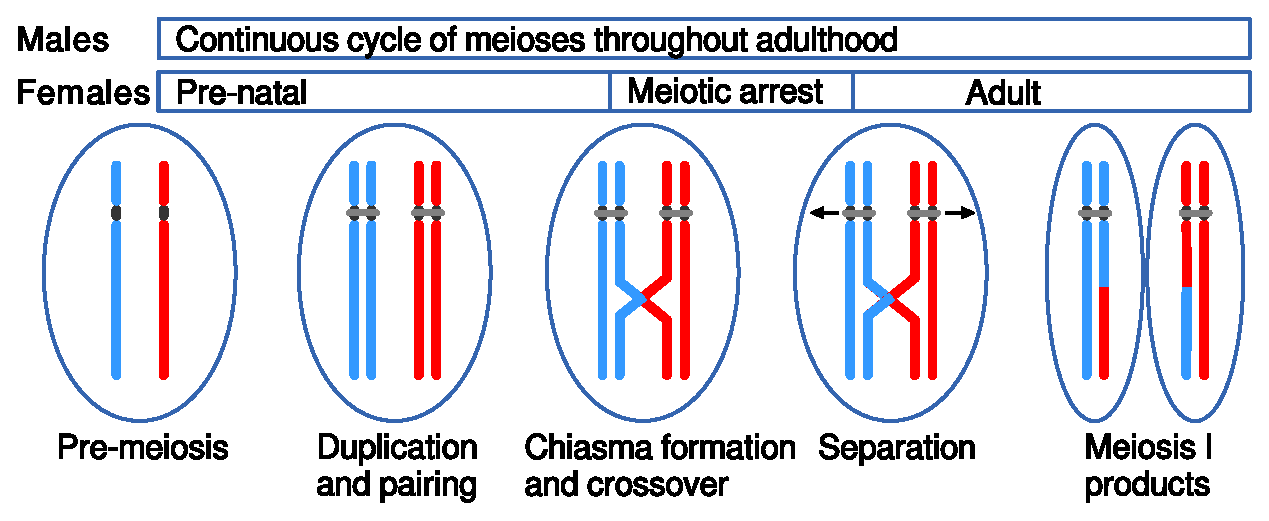
\includegraphics[width=\textwidth]{introduction/figs/meioticTiming}
    \end{center}
    \vspace{-10pt}
    \captionTitle{\textbf{Timing of meiosis I events in humans.}}{ 
        Males exhibit a continuous wave of meioses throughout adulthood.
        In females, meiosis begins before birth and enters an arrest period that can last decades before completion.
   \label{fig:introTiming}}
\end{figure}
\clearpage}

Several biological possibilities have been proposed to explain what happens to oocytes during meiotic arrest.
One is the production line hypothesis, first proposed in 1968\cite{Henderson1968}, which proposes that oocytes exit meiosis and are ovulated in the order in which they enter.
An implication of this is the oocyte produced early in the fetal stage, and thus also have an early exit, have more robust crossover connections and are less prone to aneuploidy when compared to later oocytes.
Furthermore, the production line hypothesis suggests that chiasmata frequency would decrease with age in females, as the rate of aneuploidy increases.
Several tests of the production line hypothesis have been done in mammals.
A study in mice found support for the existence of a production line in mice\cite{Polani1991}, supporting the idea that oocytes exit meiosis in the order in which they enter.
However several studies in humans contradict the assumption of a decrease in crossover count in older mothers\cite{Kong2004,Martin2015}.
Most recently, a study in over 8,000 human oocytes found no evidence for a decrease in crossover count with age.




%%%%%%%%%%%%%%%%%%%%%%%%%%%%%%%%%%%%%%%%
%%%%%%%%%%%%%%%%%%%%%%%%%%%%%%%%%%%%%%%%
\section{Historical overview of meiotic recombination}
%%%%%%%%%%%%%%%%%%%%%%%%%%%%%%%%%%%%%%%%
%%%%%%%%%%%%%%%%%%%%%%%%%%%%%%%%%%%%%%%%

% Brief historical review of meiotic recombination, pre Human Genome Project.
Recombination can be observed in a number of ways, and its discovery came decades prior to the discovery of the structure of DNA.
Thomas Hunt Morgan first observed the separation of linked traits while studying Drosophila in 1911\cite{Morgan1911}, and proposed the theory of crossing over between chromosomes.
In addition he suggested that the recombination rate could increase with the distance between factors.
Morgan's student, Alfred Henry Sturtevant, quantified this change in rate over physical distance into ``map distance,'' using this concept to construct the first genetic map.
This map represented the order of, and crossover rates between, genes on the X chromosome in Drosophila\cite{Sturtevant1913}.
In addition, Sturtevant observed that one crossover tended to inhibit the placement of a second nearby, an early description of interference.
A later study by Harriet Creighton and Barbara McClintock in corn (\textit{Zea mays}) in 1931 demonstrated that recombination between genes was tied to an exchange of chromosomal segments\cite{Creighton1931}.

Tracing the inheritance of markers from one generation to the next within a family pedigree provided the first genome-wide measurement of recombination across the human genome, prior to the completion of the Human Genome Project.
Early studies used restriction fragment length polymorphism (RFLP) probes to identify specific loci within the genome, and determine if they are linked.
An early study described the use of RFLPs to generate a linkage map of recombination in the human genome\cite{Botstein1980}.
Further linkage studies increased the marker density across the genome by using microsatellite, short tandem repeat polymorphisms (STRPs) and other approaches to capturing genetic variation\cite{Morton1991,Matise1994,Dib1996}.
The Marshfield map, generated in 1998 by \citet{Broman1998}, was an important step in characterizing recombination on a genome-wide basis.

With the completion of the Human Genome Project and the publication of the draft sequence of the human genome\cite{Venter2001,Lander2001}, human genetic variation has become increasingly well characterized, and a number of technologies have sprung up to make genome-wide ascertainment of variation routine.
Currently, microarray technology provides a well-balanced approach for determining genome-wide coverage of genetic variation.
These arrays target a pre-selected panel of hundreds of thousands to millions of single-nucleotide polymorphisms (SNPs) across every chromosome for a reasonable cost.

%%%%%%%%%%%%%%%%%%%%%%%%%%%%%%
\section{Methods for studying recombination}
%%%%%%%%%%%%%%%%%%%%%%%%%%%%%%

Genome-wide methods have the primary goal of creating a genetic map of the frequency of recombination as a function of physical distance across each chromosome.
In contrast, several other methods are limited in scope, and reveal information about specific loci.
With each method, the detection of recombination is made difficult by the fact that crossovers are rare -- only 20-50 are expected to occur in each meiosis.

% brief introduction to these before describing in detail in "description of approach"

\subsection{Pedigree analysis}

Tracking the transmission of alleles from one generation to the next within known pedigrees provided the first data on recombination in early linkage studies, and pedigree analyses are still in use today.
It is interesting to note that for a pedigree analysis, 
while whole-genome sequencing technology allows the discovery of a higher density of markers across the genome, its use is not typically worth the higher cost.
A higher variant coverage will help to narrow the region of uncertainty surrounding a particular crossover, but it will most likely not assist in the detection of additional crossovers in a single meiosis.

Regardless of the method used for obtaining markers, the principle of detecting recombination in a pedigree remains.
Crossovers can be identified by tracing the allele transmissions from parent to child.
Figure \ref{fig:introPedfig} provides a simple visual example, showing a family quartet.
The father in this pedigree has two informative SNPs producing haplotypes 1-1 and 0-0, while the mother is homozygous at both sites.
The male child has a 1-0 haplotype, and therefore must have inherited a recombinant haplotype from his mother.
We can identify here a crossover event and localize that event to an interval flanked by two informative genetic variants.
This region of uncertainty can vary in size and depends on the spacing and genotypes of polymorphic variants within the genome.
Beyond this intuitive example, the problem of determining the parental phase of a recombinant chromosome has been addressed in a number of methods.
%
\afterpage{
\begin{figure}[p]
    \begin{center}
    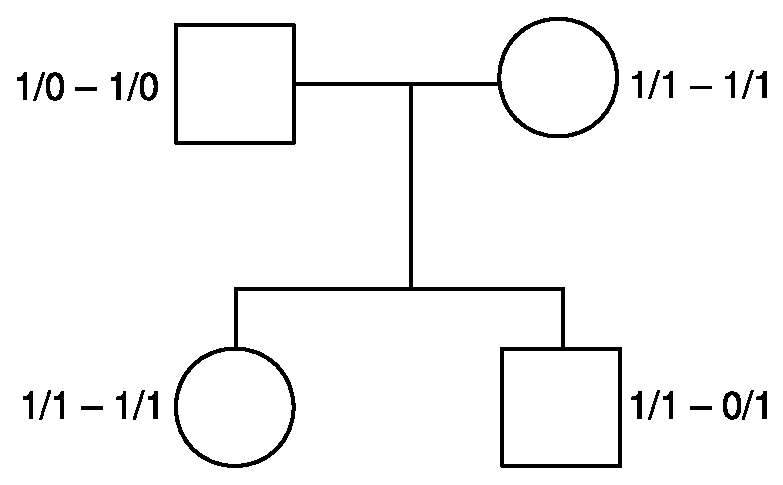
\includegraphics[width=0.75\textwidth]{introduction/figs/pedigree-genotype} \vspace{1cm} \\
    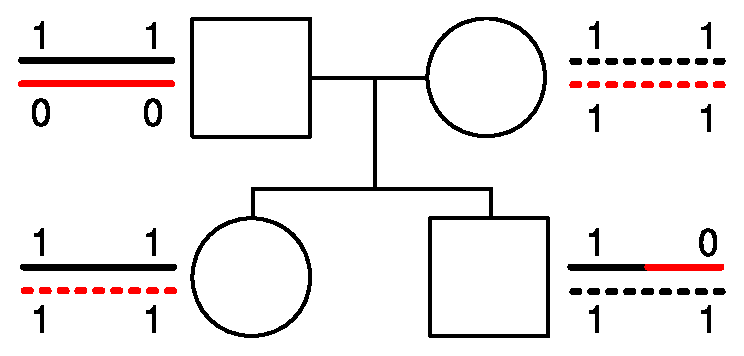
\includegraphics[width=0.8\textwidth]{introduction/figs/pedigree-haplotype}
\end{center}
    \vspace{-10pt}
    \captionTitle{\textbf{Allelic transmission in a family quartet.}}{ 
        The top panel outlines a simple pedigree in which only genotype information is known.
        The bottom panel shows a pedigree for which phase-known haplotype information is known.
        Here, all chromosomes (lines next to each individual) are transmitted in the absence of recombination except for in the male child.  Here there was a recombination event in the father to generate the recombinant chromosome (black/red)
   \label{fig:introPedfig}}
\end{figure}
\clearpage}


\subsection{Linkage disequilibrium approach}

Another powerful method is to use population genetic data to study recombination by inference.
These data can be gathered by genotyping samples of genetic data from unrelated individuals on a microarray or by whole-genome sequencing.

The inference of recombination in such a dataset relies on the quantification of levels of linkage disequilibrium (LD) within the samples, a measurement of linkage between loci.
For example, when alleles at one locus are inherited completely independently of alleles at another locus they are considered to be in linkage equilibrium.
However many alleles exhibit a non-random association, and individuals of the same species tend to share haplotype segments that reflect a shared evolutionary history.
When two alleles on an ancestral haplotype are inherited together they are considered linked, and are not independent of each other.
These alleles exhibit evidence of linkage disequilibrium, a deviation from the assumption of random assortment of alleles.

LD is measured in a pairwise fashion, considering allele frequencies at each pair of markers in the genome.


From measurements of LD within a number of unrelated samples, methods based on coalescent theory have been developed to estimate the recombination rate\cite{Auton2012}.
In software such as LDhat\cite{Mcvean2004,Auton2007,Auton2014}, the population-scale recombination rate, $\rho$, is estimated from the data, and the per-generation recombination rate can be calculated by the relationship
$\rho = 4 N_e r$
where $N_e$ represents the effective population size.
These methods are quite powerful and have produced high-quality estimates of recombination in humans\cite{hapmap2007}, however, they are subject to limitations.
First, that this method requires the knowledge of the genealogical history of a sample, which is unknown, and thus relies on an often simplistic approximation.
Second, these maps by their nature generate sex-averaged data only, since recombination events that are inferred have occurred over the course of potentially thousands of generations.


\subsection{Molecular assays}

A number of molecular assays have been developed for studying recombination.
Most, however are limited to small regions of the genome, and are more effective in males.

\subsubsection{Sperm cell assays}

Sperm typing is one method of identifying both gene conversion and crossover events.
Sperm typing was first used in 1989 to study crossing over in humans\cite{Cui1989}, and uses
allele-specific polymerase chain reaction (PCR) to identify recombination events at a given locus.
In this method, DNA is extracted from multiple haploid sperm cells from a single donor and subject to PCR.
A common reverse primer is used in conjunction with two different allele-specific forward primers, which correspond to polymorphic site in the diploid genome, and are designed to produce different amplicon sizes depending on the matching nucleotide.
Analysis of the PCR products from many sperm cells can reveal the phase of the donor individual, and the recombinant status of each sperm cell.
% \cite{Jeffreys1998,Jeffreys2000,Jeffreys2004}. % first, second(TAP2), review

Sperm typing has been used to produce high-quality data from a number of loci throughout the genome.
One of the first major findings to come out of sperm typing was the characterization of a recombination hotspot in the human major histocompatability complex (MHC), first within one gene, \textit{TAP2}\cite{Jeffreys2000}, then expanded to cover a wider 216 kb region of the MHC\cite{Jeffreys2001}.
All six hotspots found within the region of the MHC were found to be tightly correlated to regions in which LD broke down, providing molecular evidence that recombination hotpots have severe effects on LD patterns.


% Jeffreys2009: rise/fall
% Berg2010

Further work using whole genome, single-cell sequencing approaches has shed light on recombination on an individual basis for the first time.
A study by \citet{Lu2012} sequenced 99 sperm cells from an Asian male, providing valuable information on the level of variation across the entire genome of a single individual.
Here,
In addition, a further study analyzed genome-wide recombination on more than 100 sperm cells\citet{Wang2012}.
These studies are promising, and when expanded to include measurements from multiple individuals, will provide much needed data on individual level variation in crossover, and potentially gene conversion as well.


\subsubsection{Single oocytes.}
Although much harder to study, recent studies have provided much needed insight into recombination in single oocytes through novel methods.
\citet{Hou2013} conducted an analysis in human oocytes, providing at the same time a potential new method for applying next generation sequencing methods to the screening for various genetic disorders with in vitro fertilization (IVF) techniques.
Here, the researchers extracted and fertilized a total of 70 oocytes from 8 Asian female donors, collecting the first and second polar bodies, as well as the male and female pronucleus from the fertilized egg.
This complete collection of data from female oogenesis and fertilization enabled haplotype phasing and crossover calls
Most intriguingly, this enabled the generation of personal genetic maps for each donor, allowing the researchers to address the question of how recombination varies on an individual basis.
This data allows the observation of all four members of the tetrad bundle, both sister chromatids and their homologues, something usually missed by inferential studies of recombination.


Using a similar approach, recovering genetic materiel from the first and second polar bodies and oocyte, \citet{Ottolini2015} were able to observe all four products of female recombination.
The researchers generate ``MeioMaps,'' providing valuable information on how meiosis proceeds on an individual level.



\subsubsection{Recombination initiation maps}
Additional methods have been developed to identify double strand breaks within a individual cells undergoing meiotic recombination.
\citet{Pratto2014} utilized chromatin immunoprecipitation coupled with sequencing to identify DSBs associatated with the strand-exchange protein DMC1 to generate DSB maps in four unrelated human males.
This method identifies the majority of DSBs within the meiotic cell, only a fraction of which will be resolved as crossovers that could be identified via genotyping methods, the remainder ending up as non-crossover gene conversions.
The researchers found the DSB cluster into hotspots, of which 51\% overlapped with the LD crossover hotspots\cite{hapmap2007}, and 80\% of DSB hotspots overlapped regions with elevated recombination rate.
In addition, the DSB locations were largely tied to the specific PRDM9 allele for each particular individual.
PRDM9$_\text{A}$ and PRDM$_\text{B}$ alleles appear to specify similar DSB hotspots, while PRDM9$_\text{C}$ has a separate specificity.
PRDM9 heterozygosity also affects hotspot strength.


% \section{Current ``gold standard'' maps (Hapmap2 LD map, deCODE pedigree map).}
\section{Genetic maps of recombination.}

\subsection{Marshfield map}
The Marshfield map, generated by \citet{Broman1998} in 1998, was the first genetic map of the human genome at a resolution high enough to make inferences on the recombination properties in humans, using $>$8000 short tandem repeat polymorphsims (STRPs) in 188 meioses.
Here, estimates of the genome wide map lengths, inferences on individual variation, and sex differences in recombination were highlighted.
The ratio of female to male autosomal map length was estimated at 1.56, indicating that the recombination rate in females is substantially higher than males.
This ratio has proved stable over a number of studies in the intervening years (summarized in Table \ref{tab:introHeterochiasmy}).
Analysis of this this ratio as a function of chromosome position revealed that male recombination tends to be highest in the telomeres, while females had a higher ratio towards the centromeres.
This study provided valuable insight into sex dimporphism in recombination

\subsection{deCODE maps}
Another major stride in pedigree-based genetic maps came from deCODE genetics, an Icelandic pharmaceutical company that used their database of genealogical and genetic data on many Icelandic families to infer recombination, producing many high quality studies.
The first was in 2002, where 146 families, comprising 1257 meioses, were genotyped using 5136 microsatellite markers\cite{Kong2002}.
This data, in conjunction with the draft sequence of the human genome\cite{Venter2001,Lander2001} was used to improve the marker order and their placement within the reference sequence.
The genetic map generated from this study confirmed much found by \citet{Broman1998} in terms of sex dimorphism in recombination, and further characterized fine scale variation between the chromosomes.
One particular finding was that of recombination ``jungles,'' regions of high crossover rate that clustered towards the telomeres.
In addition, recombination rate was found to correlate with GC content, CpG motif occurrance, and tracts of poly(A)/poly(T), together explaining $\sim$37\% of variation.

In 2010, using genome wide SNP data on x meioses, deCODE genetics published an updated sex-specific recombination map\cite{Kong2010}.
Instead of a typical pedigree-based recombination study, \citet{Kong2010} leverage the high degree of relatedness within the Icelandic population to infer phase and parent-of-origin in 20,217 individuals typed on microarrays assaying $>$289,000 autosomal SNPs.
Here, phase is determined for parent-child pairs by taking into account haplotype blocks that are shared with other individuals within the population to determine the parent-of-origin for a particular block.
Crossovers are called when a segment of a child's haplotype is inferred to move between maternal and paternal origin.
This enables recombination be called in 15,257 parent-offspring pairs.
%%%
One effect of this parent-child phasing approach is that inference of recombination events near the telomeres is difficult, and \citet{Kong2010} omit the most distal 5 Mb for each chromosome.
The omission of the telomeric regions, where male recombination is higher, contributes to the inflation of the female:male map length ratio seen in Table \ref{tab:introHeterochiasmy}) at 1.78 in this study, however much more likely to be closer to the consensus ratio of around 1.56.
Since its release in 2010 the deCODE genetic map has proven quite valuable as a high quality sex-specific map of recombination in the human genome.


\paragraph{Other pedigree studies.}
A study in 2008 employed a pedigree analysis of individuals from the Hutterite population, all of European descent\cite{Coop2008}.
This was the first study to use genome-wide high-density SNP arrays (in this case the Affymetrix GeneChip Mapping 500k array) to study recombination.
A total of 728 meioses were analyzed, yielding valuable data regarding the overlap of crossovers and hotspots on an individual basis.
Other pedigree studies include a map generated from 980 meioses using individuals of Korean and Mongolian descent\cite{Bleazard2013}.

\subsection{Linkage disequilibrium based maps}

LD has been used to great effect in the identification of recombination events, both in the human genome and in other species.
Perhaps the most high-quality LD map comes from data generated from the International Hapmap Project, Phase II\cite{hapmap2007}, which includes data from 270 individuals genotyped at over 3.1 million SNPs.
This map was generated using samples from both European (CEU) and African (YRI) origin, greatly improving the resolution over the Phase I map.
The resolution of this map refined the collection of hotspots first identified by \citet{Myers2005}, and expands this set to include 32,996 within the human genome.
This map remains in common use today, still providing the highest resolution of sex-averaged recombination rate across the human genome.





\afterpage{
\begin{table}[p] \centering
    \begin{tabular}{|l|c|c|c|c|c|c|c|} 
        \hline Species & Common name & Study & Year & Female (cM) & Male (cM) & Ratio & Sex avg.\ (cM) \\ \hline
    \hline \end{tabular}
    \captionTitle{\textbf{Autosomal map length estimates for a number of studies in various species.}}{
    Total map lengths are given in centimorgans, while the ratio represents the female to male map lengths. Sex specific map lengths are not available for the LD based maps.\label{tab:introHeterochiasmy}}
\end{table}
\clearpage}



%%%%%%%%%%%%%%%%%%%%%%%%%%%%%%
%%%%%%%%%%%%%%%%%%%%%%%%%%%%%%
\section{Sexual dimorphism in recombination.}
%%%%%%%%%%%%%%%%%%%%%%%%%%%%%%
%%%%%%%%%%%%%%%%%%%%%%%%%%%%%%
\subsection{Heterochiasmy}

The Marshfield map\cite{Broman1998}, provided some of the first evidence of recombination rate variation across the human genome, and between males ane females.
Particularly interesting was the finding that recombination rates are higher in the telomeres, especially in males, and that females have a 1.6-fold higher rate of recombination in the autosomes.
The estimation of this ratio proved to be accurate, despite the low marker coverage and few meioses used, and has been reinforced through numerous follow-up studies\cite{Broman2000,Kong2002,Coop2008,Kong2010,Bleazard2013,Campbell2015,Bherer2016}.

This example in humans provides an illustration of heterochiasmy, the unequal distribution of recombination rates between the sexes of a species.
Humans are among a large majority of species with data currently available in which the female recombination rate is higher than that of the male (Table \ref{tab:introHeterochiasmy}).


Haldane-Huxley rule: when recombination is absent in one sex, it is the heterogametic sex.
%
Trivers hypothesis: recombination is lower in the sex that undergoes stronger selection (recombination disrupts favorable haplotypes in the most fit individuals, therefore is selected against).

%%%%%%%%%%%%%%%%%%%%%%%%%%%%%%
\subsection{Maternal age effect.}
%%%%%%%%%%%%%%%%%%%%%%%%%%%%%%

Age effects on reproduction have been tied with an increased incidence of aneuploidy in humans\cite{Hassold2001,Hassold2007}.

Several studies have shown evidence for an increase in the number of crossover events with maternal age, suggesting a protective mechanism against aneuploidy.
%%%
With the aim of investigating age effects in recombination, a study in 2004 using the deCODE genetics dataset with 23,066 meioses, using a reduced set of 1000 microsatellite markers\cite{Kong2004}.
Genotyping was not done for every individual, with some families having only one parent genotyped, and recombination events were therefore imputed.
The main finding from this study is that the number of crossovers observed in females appears to increase with age, with an additional 0.082 events per year ($\pm$0.012), corresponding to a 4\% increase over 25 years.
This effect was seen to increase within families, such that a child born later in the mother's life has a higher number of maternal crossover than their siblings born earlier.
\citet{Coop2008} analyzed recombination in 728 meioses from Hutterites, and found that mothers 35 year or older have an extra 3.1 crossover events compared to mothers under 25 years old.
This effect corresponds with an extra 0.19 events per year ($\pm$0.092).
No such effect was found in males in either study.
%%%

A study by \citet{Hussin2011} examined in recombination in 195 maternal meioses from French-Canadian pedigrees.
Here, the opposite effect was seen, with recombination rate found to decrease with maternal age, with a larger effect size, estimating a decrease somewhere between $-$0.49 and $-$0.42 events each year.
Differences in the direction of the effect here may be due to real differences between populations, when considering the French-Canadian as a genetic isolate, or simply due due to a lack of power with only 195 meioses.
%%%
Another study reported a slight decrease in crossover count with maternal age in 338 meioses, finding a decrease of $-$0.29 events per year\cite{Bleazard2013}.
In a direct test of the production line hypothesis, \citet{Rowsey2014} examine more than 8,000 oocytes, finding no significant change in crosover count among oocytes.
Thus, it appears that the number of crossovers in a given oocyte is not governed as a function of order of meiotic entry, and there is a lack of evidence for any effects of the production line hypothesis on crossover count.

While evidence for an age effect on crossover count in females is conflicting, these studies all agree that there is no age effect present in males.
A recent meta-analysis by \citet{Martin2015} provided much need insight into the age effect issue.
Using a combination of nine cohorts comprising $>$6000 meioses, the authors report a modest but significant increase in the crossover count with age.
The authors used a comprehensive and systematic approach that avoids the methodological differences between previous studies.
%%%
An interesting suggestion from this study, was that of possible confounding factors upon the maternal age effect.
One, that assisted reproductive technologies, including IVF, may provide an artificial selection for oocytes with a greater number of crossovers.
Second was the possibility that oral contraception, which suppresses ovulation, could somehow alter the age-count association, especially if the production-line hypothesis holds true for humans.
However, neither of these possibilities could be controlled for with the power of this study and remain undetermined.


Additional evidence from an analysis of single oocytes provides evidence that maternal recombination rate is highly variable within a single individual, with 41.6 $\pm$ 11.3 crossover per oocyte\cite{Ottolini2015}.
This study revealed a selection against transmission of non-recombinant oocytes at meiosis II, which were more likely to be found in the second polar body instead of the transmitted oocyte.
This evidence outlines a potential mechanism by which non-recombinant, potentially aneuploid oocytes could be eliminated from the germ line.
Furthermore, recombination, thought to be limited to prophase I, was shown to influence events in meiosis II, much later than previously thought.

%%%%%%%%%%%%%%%%%%%%%%%%%%%%%%%%%%%%%%%%
%%%%%%%%%%%%%%%%%%%%%%%%%%%%%%%%%%%%%%%%
\section{Hotspots}
%%%%%%%%%%%%%%%%%%%%%%%%%%%%%%%%%%%%%%%%
%%%%%%%%%%%%%%%%%%%%%%%%%%%%%%%%%%%%%%%%

\subsection{Initial discovery of hotspots}

Sperm typing produced the first set of well-characterized hotspots in humans, initially focusing within the MHC\cite{Jeffreys2000,Jeffreys2001}.
The correlation of hotspot locations identified by sperm typing in this regions with breakdown of LD measurements provided support for the use of LD methods to find hotspots of recombination genome-wide, without the expense and limitations of single-cell assays\cite{Jeffreys2001}.
In 2005, \citet{Myers2005} produced a fine-scale recombination map in the human genome using LD methods.
Along with this map, hotspots were found to be a ubiquitous feature of the human genome, with a set of $\sim$25,000 found, occurring roughly every 50 kb.
Hapmap LD study expand characterized hotspots throughout the human genome.
These LD studies of recombination also estimated the proportion of recombination occurring within various fractions of the total genome sequence, finding that recombination was intensely concentrated, with 80\% of all recombination occupying less than 20\% of sequence.

Extensive analysis by sperm typing has indicated that hotspots are generally 1-2 kb in width\cite{Jeffreys2004a,Arnheim2003}.


\subsection{Discovery of PRDM9}

Since hotspots were first looked at in detail, and the discovery that they were common and spread across the entire genome, questions regarding a possibly regulatory mechanism for hotspots have persisted.
\citet{Myers2005} found that hotspots shared many common features including repeat elements THE1A/B, and a common sequence motif (CCTCCCT) located at the centers of many hotspots.
A further famly of motifs were identified via the use of the Hapmap phase 2 LD map\cite{hapmap2007}, encompassed by the degenerate 13 bp motif (CCNCCNTNNCCNC)\cite{Myers2008}, estimated to be involved in up to 40\% of all hotspots.

Spencer2006 : hotspots associated with increased GC content, and GC increasing mutations, a likely result of the action of biased gene conversion.


In 2010, a series of papers by three separate groups converged on the identification of PRDM9 from different approaches.
This protein, originally called \textit{Meisetz} was discovered in mice, and is active in early meiotic prophase\cite{Hayashi2005}.
PRDM9 contains a high polymorphic zinc finger DNA binding array, as well as a methyltransferase domain, responsible for the trimethylation of lysine 4 on histone 3 (H3K4).

\citet{Myers2010} compared the sequence of the 13 bp motif against predicted binding of various zinc finger arrays in the genome, finding PRDM9 as a top candidate.
%predicted binding sequence of the PRDM9 zinc-finger array in humans, they found that PRDM9 is a match for the 13 bp sequence motif found at the center of human hotspots.
%Looked at the recombination rate in chimpanzees in sequence surrounding human hotspotso
Using a mouse genetic approach, \citet{Baudat2010} focused on a locus previously determined to be involved in localization of crossover initiation\cite{Grey2009,Parvanov2009},
and narrowed this genomic interval to a region containing the \textit{Prdm9} gene.
A third study used fine mapping techniques in mice to narrow the region, again identifying PRDM9 as the likely candidate protein\cite{Parvanov2010}.

\subsection{PRDM9 alleles}

The PRDM9 zinc finger array has tremendous variability and there are a number of alleles present.
The major alleles A and B, are both present in a high percentage of European individuals, and differ by only a single amino acid change\cite{Baudat2010}.
The A and B alleles are predicted to recognize the degenerate 13-mer motif, but the I allele is not\cite{Baudat2010}.
This effect is seen at the DSB-level as well, with PRDM9 A and B variants contributing to generate silmilar DSB hotspots\cite{Pratto2014}.

Furthermore the PRDM9 allele status of an individual has a strong effect on the hotspot overlap.
In the Hutterite study, A/A individuals have significantly different overlap compared to A/I, and A/B, with the A/I heterozygous having lower hotspot usage overall\cite{Baudat2010}.


Sperm typing in men of African ancestry revealed that PRDM9 variants similar to the ``C'' allele (termed C-type), were more common in this population.
Furthermore, these C-type alleles specified different hotspots with a motif different from those seen Europeans\cite{Berg2011}. 
These ``African-enhanced hotspots'' all contained a common motif, CCNCNNTNNNCNTNNC, but were associated with the PRDM9 C-type alleles.




\subsection{Hotspots in other species}

Hotspots have been discovered in a number of other species.

Mice contain approximately 15,000-20,000 hotspots, also under the regulation of PRDM9
Mice: Brick2012 (Hotspots via ChIP); Smagulova2011. 15-20,000 total

PRDM9 absent / present

Dogs (Axelsson, Auton2013)

Yeast

Birds


\subsection{Conservation between species}

Humans and chimpanzees have a complete absence of hotspot sharing, despite a high degree of overall DNA sequence identity\cite{Ptak2005,Winckler2005,Auton2012a}.

Evidence points the rapid evolution of the zinc finger DNA binding array as an explanation for the lack of shared hotspots between humans and chimpanzees\cite{Myers2010}, and a wide variety of mammals\cite{Oliver2009,Ponting2011,Thomas2009}.

Discuss hotspot paradox vs stable hotspots theory (latter saying hotspots are confined to specific chromosome features (promoters/GC content), as in yeast and dogs)

\subsubsection{Species lacking PRDM9}
Dogs, birds (Singhal2015, biorxiv) 

%%%%%%%%%%%%%%%%%%%%%%%%%%%%%%%%%%%%%%%%
%%%%%%%%%%%%%%%%%%%%%%%%%%%%%%%%%%%%%%%%
\section{Determinants of recombination placement within the genome.}
%%%%%%%%%%%%%%%%%%%%%%%%%%%%%%%%%%%%%%%%
%%%%%%%%%%%%%%%%%%%%%%%%%%%%%%%%%%%%%%%%
% Differences in populations (Berg2010,Berg2011,Hinch2011)


\subsection{Distribution within the genome}

The distribution of recombination within the genome has been shown to vary considerably between individuals, sexes, and populations.
At the broad scale, crossovers are not distributed equally across the genome.
The recombination rate is higher towards the telomeres\cite{Broman1998,Mcvean2004,hapmap2007}.
This effect seems to be primarily driven by males, with crossover occurring more frequently in telomeric reions, while females have higher recombination rates closer to the centromeres\cite{Kong2002,Coop2008,Kong2010}.

Numerous studies in humans have found that recombination tends to be depressed within gene regions overall, with recombination high just upstream and downstream of gene regions\cite{Mcvean2004,Myers2005,hapmap2007,Spencer2006,Kong2010}.
In addition, when looking further away from gene regions, around 500 kb away, recombination appears to be elevated, then falling off after a few hundred kb.

Evidence for sex differences in recombination has also been suggested to occur around gene regions.
\citet{Kong2010} found that recombination was lower within genes overall, and that
female recombination was lower within genes, but higher in the surrounding regions.
Additionally, while females have a lower rates within genic regions, males have higher rate within exonic regions.

In addition, results from LD maps in humans have examined the proportion of recombination occupying various proportions of sequence.
From these analyses, it is estimated that the majority of recombination, 80\%, occurs in approximately 20\% of the sequence\cite{Mcvean2004,Myers2005,hapmap2007}
This concentration of recombination could be due to clustering within hotspots.
A majority of crossovers in each meiosis were found to cluster into recombination hotspots, driving recombination into limited region of the genome\cite{Coop2008}, although this overlap varies widely between individuals.


\subsection{Recombination under genetic control}
% Genes involved in recombination (RFN212, etc)}

A number of genetic factors have been identified that alter properties of recombination, a summary of which can be found in Table \ref{tab:introGenes}.

In a sperm typing analysis, \citet{Jeffreys2005} found a SNP whose minor allele suppressed the ratio of crossover to gene conversion near a particular hotspot.
Additionally, this variant was found to be overtransmitted, an example of meiotic drive.
Another study in the Icelandic population found an association with an inversion at 17q21.31 on recombination rate\cite{Stefansson2005}.
The presence of this inversion is associated with an increase in crossover rate in females, but not males.

% RNF212: indentified in Saccharomyces cerevisiae and Caenorhabditis elegans
RNF212 has been associated with recombination rate in an Icelandic population\cite{Kong2008}, and this has been replicated in a number of follow-up studies\cite{Chowdhury2009,Fledel-Alon2011,Reynolds2013,Kong2014}.
Interestingly, the linkage of two particular SNPs near this gene is associated with an increased recombination rate in males, and a corresponding decreased rate in females.
RNF212 is a homologue of ZHP-3, a \textit{C.\ elegans} gene involved in crossing over and disjunction, localizing to sites of crossover, and aids in the change in chromatin structure that occurs with the disassembly of the synaptonemal complex\cite{Bhalla2008}.
Mouse RNF212 was found to have similar function, facilitating synapsis, and forming crossover-stabilizing structures\cite{Reynolds2013}.
%Rnf212 KO mice are sterile but achieve complete synapsis.
In addtion RNF212 possibly influences the decision to repair a DSB as a crossover rather than a gene conversion\cite{Reynolds2013}.

A study by \citet{Chowdhury2009} using 2310 meioses found significant associations with variants associated with four gene regions.
Two were associated with female recombination rate (KIAA1462, PDZK1), and the other two with male rate (UGCG, NUB1).
These genes are poorly characterized and their function, beyond potential meiotic roles, remains unknown.
However, this study reinforces the suggestion that male and female recombination rate are controlled via differing genetic factors.

Another study, again in the Icelandic population with an expanded number of meioses, identified a further 8 genomic regions that have separate associations with male and female rates\cite{Kong2014}.
In the telomeric region of chromosome 4, near RNF212, one variant was found that was estimated to increase the map length by 386 cM in females, and 124 cM in males.
Novel variants were found in an additional six genes (Table \ref{tab:introGenes}).

The strongest association thus far has been with PRDM9, which was first associated with hotspot usage and variation in alleles encoding the zinc finger array\cite{Baudat2010,Berg2010}.
\citet{Berg2011} found that variation in PRDM9 alleles greatly influences hotspot usage in African populations, who appear to have a distinct subset of hotspots\cite{Hinch2011}.
Genome-wide associations with hotspot usage were replicated in the Icelandic population with strong effects\cite{Kong2010}.

In non-human studies, both RNF212, and REC8, a SC-associated protein, have also been shown to associate with recombination rate in cattle\cite{Sandor2012}.

\afterpage{
\begin{table}[p] \centering
    \small
    \begin{tabular}{|l|c|c|p{1.3cm}|p{1.3cm}|c|c|} 
\hline Gene / region & Chr. & Association & Female rate & Male rate & Study & Replication \\ \hline
        RNF212 & 4 & rate & + & - & \citet{Kong2008} & \cite{Chowdhury2009,Fledel-Alon2011,Reynolds2013,Kong2014,Campbell2015} \\
        17q21.31 inversion & 17 & rate & + & none & \citet{Stefansson2005} & \cite{Fledel-Alon2011,Chowdhury2009,Kong2014} \\
        KIAA1462 & 10 & rate & + & none & \citet{Chowdhury2009} &  \\
        PDZK1 & 1 & rate & + & none & \citet{Chowdhury2009} &  \\
        UGCG & 9 & rate & none & + & \citet{Chowdhury2009} &  \\
        NUB1 & 7 & rate & none & + & \citet{Chowdhury2009} &  \\
        CCNB1IP1 & 14 & rate & + & weakly + & \citet{Kong2014} & \cite{Campbell2015} \\
        C14orf39 & 14 & rate & + & none & \citet{Kong2014} &  \\
        SMEK1 & 14 & rate & + & none & \citet{Kong2014} & \cite{Campbell2015} \\
        RAD21L & 20 & rate & weakly + & + & \citet{Kong2014} &  \\
        MSH4 & 1 & rate & + & none & \citet{Kong2014} &  \\
        CCDC43 & 17 & rate & + & none & \citet{Kong2014} &  \\
        PRDM9 & 5 & hotspot usage & NA & NA & \citet{Baudat2010} & \cite{Fledel-Alon2011,Campbell2015,Kong2014} \\
    \hline \end{tabular}
    \captionTitle{\textbf{Genomic regions associated with recombination in humans.}}{
    \label{tab:introGenes}}
\end{table}
\clearpage}


\subsection{Heritability of recombination modifiers}

The 2004 deCODE study, by analyzing siblings in large families, suggested that recombination rates were broadly heritable\cite{Kong2004}.
The pedigree analysis of the Hutterize population by \citet{Coop2008} was the first to find extensive variation among individuals in terms of their hotspot overlap (the proportion of an individual's crossover that overlap with known hotspots).
Another significant finding was that hotspot overlap was heritable.
This raises the possibility that other aspects of the recombination process may also be heritable.
And supports previous data from sperm typing finding that a hotspot-proximal SNP had recombination-suppressing effects, and that this SNP is over-transmitted to progeny\cite{Jeffreys2005}.

A follow-up study in 2011 reinforced the heritability of hotspot usage as a phenotype, and expanded the scope\cite{Fledel-Alon2011}.
This study found that both male and female recombination rates are heritable.
Additionally, associations with RNF212 and the inversion on 17q21.31 were replicated.

% Ottolini2015: selection for maternal recombination rates. (Kong2004 suggested this as well).
%\section{Heritance of recombination modifiers (rate, etc. Kong)}



%%%%%%%%%%%%%%%%%%%%%%%%%%%%%%%%%%%%%%%%
%%%%%%%%%%%%%%%%%%%%%%%%%%%%%%%%%%%%%%%%
\section{Recombination in other organisms}
%%%%%%%%%%%%%%%%%%%%%%%%%%%%%%%%%%%%%%%%
%%%%%%%%%%%%%%%%%%%%%%%%%%%%%%%%%%%%%%%%


Recombination in humans is of great interest to us as a species, and much effort has been focused here.
However it is of great interest to learn about recombination in all species to put human recombination in an evolutionary context.
Studies of recombination have been done in a wide variety of organisms to date, a partial list of which is summarized in Table \ref{tab:introHeterochiasmy}.

Chimpanzees, the most recent common ancestor to humans, have a LD-based recombination map\cite{Auton2012a}, but no pedigree maps are yet available, leaving open questions regarding sex differences.

Pedigree maps have been generated in mice\cite{Broman2002}, the most recent of which 
was generated by \citet{Cox2009}, using 3546 meioses, but a low density of markers.
More recently, data from the Collaborative Cross(citation), an inbred population generated from eight founder strains, has been used to generate sex-specific maps within the mouse genome\cite{Liu2014}.
The researchers here leveraged the breeding funnel approach from the Collaborative Cross, gathering genotype data from sibling pairs, and using computational techniques to infer recombination events.


Yeast has been the subject of a number of studies, due to their ease of use as a model organism and much of what we know today comes from yeast.

Recombination maps are available in a number of other species, but most are limited to LD studies, due to the steep resource requirements of pedigree studies.
Most recently, study of recombination was released in yeast\cite{Lam2015} and birds\cite{Singhal2015}.
These studies provided an evolutionary perspective on recombination initiation and hotspot evolution.



%%%%%%%%%%%%%%%%%%%%%%%%%%%%%%%%%%%%%%%%
%%%%%%%%%%%%%%%%%%%%%%%%%%%%%%%%%%%%%%%%
\section{Recombination and disease}
%%%%%%%%%%%%%%%%%%%%%%%%%%%%%%%%%%%%%%%%
%%%%%%%%%%%%%%%%%%%%%%%%%%%%%%%%%%%%%%%%

The most direct association of recombination with disease is the association with aneuploidy due to meiosis I errors\cite{Hassold2001,Hassold2007}.
As recombination has such a high impact on the structure of the genome, it also has the possibility to cause genomic instability if errors occur during the break and repair of DNA.
Defects in recombination have been associated with a number of disorders caused by genomic instability.
Nonallelic homologous recombination (NAHR), also known as ectopic exchange results in structural genomic rearrangements and is a major cause of recombination-associated copy number alteration.
For example, 22q11.2 deletion syndrome is believed to be caused by improper pairing and crossing over between low copy repeats (LCRs) that flank the region, causing it to be deleted in the recombinant chromosome\cite{Emanuel2008}.
Ectopic exchange contributes to a number of other diseases associated with genomic rearrangements\cite{Stankiewicz2002,Liu2012}.
\citet{Berg2010} reported that variation found at the PRDM9 locus contributed to genome instability.
\citet{Pentao1992} found that rearrangements between repeat regions associate with the the deleteion of a 1.5 Mb region, associated with Charcot-Marie-Tooth disease type 1A (CMT1A).
Deletion of the 7q11 region in sperm causes Williams-Beuren syndrome\cite{Turner2008}.

PRDM9 has also been implicated in genomic instability associated disease.
PRDM9 hotspot motifs have been found in regions associated with disorders of genomic instability\cite{Myers2008}.
In a sperm-typing study, non-A alleles of PRDM9 were found to be protective against the risk of rearrangements leading to CMT1A and hereditary neuropathy with liability to pressure palsies (HNPP)\cite{Berg2010}.
Here, a protective effect against genome rearrangement was seen in men homozygous for the N/N allele, with a lesser effect in heterozygous A/N individuals.

In addition, PRDM9 has been associated with children with B-cell precursor acute lymphoblastic leukemia (B-ALL)\cite{Hussin2013}.
Here, a rare PRDM9 allele (C) was found in a number of families, and was tied to the abnormal X of crossover events, and associated with B-ALL.

%Berg2011:

However, an interesting recent study identified a healthy mother carrying a homozygous knockout of PRDM9 predicted to render the protein inactive\cite{Narasimhan2016}.
In PRDM9 knockout mice, meiosis is not able to complete properly\cite{Brick2012}.
However, this mother had three healthy children, one of which carried the mutation.
In this transmission, crossovers at PRDM9 binding locations reduced in number.
This observation by \citet{Narasimhan2016} raises the possibility of a backup mechanism for the completion of meiosis in the absence of PRDM9 in the human genome.

%%%%%%%%%%%%%%%%%%%%%%%%%%%%%%%%%%%%%%%%
%%%%%%%%%%%%%%%%%%%%%%%%%%%%%%%%%%%%%%%%
\section{Interference}
%%%%%%%%%%%%%%%%%%%%%%%%%%%%%%%%%%%%%%%%
%%%%%%%%%%%%%%%%%%%%%%%%%%%%%%%%%%%%%%%%

%%%%%%%%%%%%%%%%%%%%%%%%%%%%%%%%%%%%%%%%
\subsection{Crossover interference}
%%%%%%%%%%%%%%%%%%%%%%%%%%%%%%%%%%%%%%%%

% Current status of crossover interference field.
Crossover interference, also known as chiasma interference, is another mechanism that affects the placement on crossover events on a chromosome.
Interference was first observed in flies in 1913\cite{Sturtevant1913}, but not formally named until 1916 when Hermann Muller coined the term:
\begin{quote}
    In a sense, then, the occurrence of one crossing-over interferes with the coincident occurrence of another crossing-over in the same pair of chromosomes, and I have accordingly termed this phenomenon ``\textit{interference}''.
%\hfill Hermann J Muller, 1916\cite{Muller1916}
\end{quote}
%
When two or more events occur on the same chromosome during the same meiosis, crossover interference effects the spacing of events.
Positive interference causes events to be placed further apart that expected, while negative interference results in events being placed closer together.
Under positive interference one crossover occuring on a chromosome is thought to ``interfere'' with a second, and inhibit its placement nearby.
Crossover inteference affects the linkage patterns between genes, has possible implications for ensuring disjunction of chromosomes.



% potential method of coint action.
% Cover what's known in humans, dogs, other organisms.
% genetic map functions taking into account coint Speed,Zhao

\subsubsection{Biological models of crossover interference}

Several biological explanations have been proposed to account for the action of crossover interference in the genome, and are reviewed here.
An early suggestion was that steric interference was responsible for interference.
In this case, a cluster of proteins that are necessary to facilitate resolution of the DSB would bind, the prevent further attachment at nearby sites.
This idea was mostly discounted after cytological studies failed to observe complexes of a sufficient size to enable interference over long enough distances.

One aspect that models seek to address is that of crossover homeostasis, and crossover assurance.
Crossover assurance captures the idea that as least one crossover is required per chromosome, which is thought to prevent non-disjunction.
In a typical meiotic progression, multiple DSBs are created in the DNA and only a small fraction of themresolve to crossovers, with the remainder repaired as non-crossover gene conversions.
Studies in yeast have shown that the final number of crossovers remains at the same level even when reducing the number of precursor DSBs\cite{Martini2006}.
Thus, it appears that there is some regulatory mechanism in place to ensure at least one crossover per chromosome.
Another implication of crossover homeostasis is that it has the potential to change the ratio of crossovers to gene conversion events.
Since crossovers tend to be maintained at a constant level, the number of gene conversions decreases.


%%% crossover homeostatis
%%% crossover assurance

\paragraph{The mechanical stress model.}
\citet{Kleckner2004} proposed a model in which interference is governed by mechanical forces.
This model starts from the basis that chromatin configuration changes over the course of meiosis, undergoing expansion and contraction cycles.
These expansions and contractions create waves of periodic increased or decreased stress that propagate along the chromosome.
DSBs create ``cracks'' in the DNA, reducing the amount of stress directly near the crack.
The amount of relief slowly decreases with greater distance away from the break until the stress returns to normal levels.

This model has a number of properties that fit into generally accepted properties of recombination.
First, it ensures that at least one crossover will occur on each chromosome, as long as enough stress is generated.
Second, it allows for specification of the location of stress and therefore DSBs and crossover, based on, for example, chromatin configuration.
Finally, this model allows for interference to act at multiple time points in meiosis using the same mechanism.
However, the mechanical stress model assumes that all crossovers are interfering, and does not explain the observation that some organism appear to have two pathways of interference.

\paragraph{The polymerization model.}
The polymerization model describes the maturation of DSBs to crossovers in terms of a time-dependent polymerization event spreading along the synaptonemal complex\cite{King1990}.
The progression of DSBs to chiasmata to mature crossovers is described in terms of a precursor structure binding, triggering this maturation.
In the model, early recombination precursors form randomly along the chromosome while it is tied into the synaptonemal complex.
Some of these early events mature into chiasmata and become crossovers.
As this maturation occurs, a polymerization event is triggered that moves in both directions away from the crossover.
The expanding polymer blocks the binding, or forces detachment, of further precursor structures that would lead to crossover, thus creating an interference effect.
The ejected precursors could then re-bind at another location on the chromosome.

This model makes a distinction between early and late crossover events, guarantees at least one crossover occurs, and captures the distance-dependency of the interference effect.
However, no evidence of a polymer structure has been observed in cytological studies.
Furthermore, studies in mice have shown that the synaptonemal complex is not required for interference to act\cite{DeBoer2007}.

\subsubsection{Mathematical models of crossover interference}

\paragraph{The counting model.}
The counting model does not depend on SC length, but instead proposes that crossovers must be separated by a discrete number of non-crossover gene conversion in between\cite{Foss1993,Foss1995}.
In this model, a fixed number of events (presumed to correspond to DSBs) are placed randomly upon a chromosome.
Then, the events are classified in one of two ways, either crossovers or gene conversions.
Crossovers form the minority of the mature events with a specific number of gene conversion in between.
Therefore, no two crossovers can occur directly beside one another, and some degree of distance-dependent spacing is maintained.

Data in Drosophia were found to fit this model well, it was found that it poorly predicted interference in budding yeast and humans\cite{Foss1995}.
Therefore, extensions to this model were made to allow a second class of non-interfering crossovers to exist along-side those that are interfereing (see ``The simple gamma model'' on page \pageref{cointTPM}).

A key element of the counting model is that interference here depends on genetic distance rather than physical, or SC distance.
This allows interference to be estimated in different species with differing genomic properties, such as chromosome size.
This also serves to to ``normalize'' the enormous differences in recombination rates per physical distance that are seen in nature.
Even within species, due to sex-differences in recombination rate, any comparison between males and females must be done using the genetic position (in cM) of each crossover, which takes into account differences the genetic map length.

% \paragraph{Chromosome oscillatory movement model.}


%gamma and two-pathway model, math review.
% \paragraph{The count-location model.}
% \citet{Broman2000} tested several versions of the count-location model of interference against early genome-wide data from humans.

\paragraph{The simple gamma model.} \label{cointTPM}

The gamma model starts with the assumption that all crossovers are capable of interfering with each other, and chromatid interference is neutral.
The location of chiasmata on a tetrad bundle are determined by a stationary renewal process(*).
The inter-chiasmata distances are are modeled to follow a gamma distribution with a single parameter, $\nu$, representing the strength of interference.
In this model, $\nu <$ 0 corresponds to negative interference, $\nu=$ 0 no interference, and $\nu>$0 positive interference.
The shape and rate parameters of the gamma distribution are not independent, but instead represented with shape of $\nu$ and rate 2$\nu$.
Therefore, the gamma distribution has a mean of 0.5 Morgans, and a standard deviation of $1 / ( 2 \sqrt{\nu} )$.


In typical recombination studies, the locations of the chiasmata are unknown and only the crossover locations are observed.
From a four strand tetrad, crossing over occurs twice as often as what is observed on a single product, so chiasmata are thinned to become crossovers.
Since chromatid interference is neutral, each chiasma has a 0.5 probability of becoming a crossover.
The mean inter-chiasma distance of 0.5 therfore translates into an average distance of 1 Morgan between crossovers.

This model allows crossover locations from transmitted genotype data to be used to estimate the parameters of a gamma distribution that represent the strength of crossover interference.




\paragraph{The two pathway model.}

The two pathway model is an extension of the gamma model that allows a non-interfering crossovers to exist in a mixture with those that are affected by interference.
After a growing body of data suggesting that there may be two distinct pathways of crossing over in a number of humans, \citet{Housworth2003} proposed the two pathway model of interference in 2003.

Here, the gamma model is extended to a mixture model.
The class of interfering crossovers continue to be represented by the gamma distribution with a positive $\nu$, and the non-interfereing crossovers by a simplified gamma distribution where $\nu=$1.
A second parameter is added, $p$, which controls the mixture between these two cases.
Interfering crossovers occur with proportion $(1-p)$, and non-interfering crossovers with proportion $p$.
Thus, $p$ represents the proportion of non-interfering crossover in the distribution.
These crossovers are said to ``escape'' the effects of crossover interference.

\subsubsection{Data on crossover interference}

\paragraph{Cytological measurement of interference}
A cytological study in mice measured distances between foci marking crossover events in terms of relative distance along the SC, and models these distances using a gamma distribution\cite{DeBoer2006a}.
The researchers looked at MLH1 foci, which mark crossovers at the pachytene stage, as well as MSH4 loci, which occur just prior, in the zygotene stage.
Positive interference was observed in both foci at both stages, however it was much stronger in the later staage, marked by MLH1 foci at pacytene.
A follow-up to this study found that interference was not affected by the lack of an intact SC, and that interference remained present even without complete synapsis\cite{DeBoer2007}
Furthermore, interference between x foci indicate that interference can act between DSBs and is not limited to the subset that resolve as crossovers\cite{Baudat2007}.

These studies suggest that, at least in mice, interference acts across at least two stages of meiotic prophase, and is not dependent on the full assembly of the synaptonemal complex.
Furthermore, these observations appear to support the mechanical stress model of interference.

Since this study, this method has been used in number of other organisms\cite{Barchi2008,Basheva2008}.
% \cite{Barchi2008,Basheva2008,Vozdova2013,Borodin2008,Borodin2008b,Borodin2009,Mary2014}
% Barchi2008: mice.  cytological interference is reduced in ATM KO mice.
% Basheva2008: dogs. positive COint, nu=6.5
%%% Table on cytological interference?
%
Many of these found similar levels of crossover interference, suggesting that interference is a conserved feature.

\paragraph{Strength across the genome.}
A cytological study of crossover interference in human males\cite{Lian2008} found that interference strength was high in smaller chromosome, and decreased with larger chromosomes.
However, this data was re-analyzed by \citet{Housworth2009}, this time using the two-pathway model, who found that interference strength was constant across all chromosomes.


%%%%%%%%%%
% Interference in yeast: NCO has no interference\cite{Baudat2007}?.
% Getz2008: support two pathway model of interference., and contradit Baudat2007, suggesting that interference acts in two pathways, and that either can result in a CO or NCO (in yeast).

% The finding that interference can act between DSBs in mice\cite{Baudat2007} suggests that interference may affect the placement of gene conversion events as well.
%%%%%%%%%%

\paragraph{Interference inferred from pedigree studies.}

The centromere is not a barrier to interference\cite{Broman2000,Fledel-Alon2009}, and acts over the entire chromosome.

The recombination initiation maps generated by \citet{Pratto2014} provided important data regarding the initiation of DSBs that will lead to crossover events.
One suggestion from this study is that interference could act between nearby hotspots, inhibiting the formation of a second DSB nearby, supporting the idea DSB-DSB interference found in mice.

The crossovers identified from single oocytes by \citet{Hou2013}
allows valuable data to be inferred regarding both crossover interference, affecting the spacing between pairs of crossovers.
Comparing to previously published sperm data\cite{Lu2012}, \citet{Hou2013} look at crossover spacing as a function of both physical distance (in bp), and synaptonemal complex length (\SI{}{\micro\metre}), concluding that the strength of interference is equivalent in males and females when considering the synaptonemal complex length, which is longer in females, reflecting their higher recombination rate.
%an observation that conflicts with a number of other studies\cite{Broman2000,Housworth2003,Fledel-Alon2009}.
Somewhat puzzling was the omission of genetic distance (in centimorgans) in this analysis, a factor that controls for the 1.6 fold higher recombination rate in females over males.
A reanalysis of this data using genetic distance is presented in this thesis in Chapter \ref{cointExtras}.


\subsubsection{Other methods of measuring coint}
Coefficient of coincidence.
% The ratio of probability

%%%%%%%%%%%%%%%%%%%%%%%%%%%%%%%%%%%%%%%%
\subsection{Chromatid interference}
%%%%%%%%%%%%%%%%%%%%%%%%%%%%%%%%%%%%%%%%

Another type of interference that is somewhat more difficult to observe, and therefore less studied, is chromatid interference.
Chromatid interference affects which chromatid is involved in crossing over within the tetrad.
Chromatid interference occurs when a crossover between two chromatids changes the probability of those same two chromatids to be involved in further crossover during the same meiosis.
%In theory, recombination is only effective when it occurs between homologues.
%Exchange of identical segments between sister chromatids serves little purpose with respect to the reshuffling of alleles on a chromosome.

By identifying which chromatid is involved in each crossover \citet{Hou2013} found evidence for weak and negative chromatid interference in human oocytes.
This means that once an initial crossover is established between two chromatids (e.g.\ labeled 1 and 2), a second crossover is more likely to form using at least one of these first chromatids (1 and 2), and less likely to form using neither (between 3 and 4).
Positive chromatid interference corresponds to an decrease in the probability of a second crossover involving the same chromatids as the first, that is, the first crossover ``interferes'' or prevents the placement of the second on the same chromatids.

In another study, \citet{Fledel-Alon2009} used the observed crossovers to infer the chiasma count in tetrads using human pedigrees.
Under their model, chromatid interference could account for the observed transmission of nullichiasmic, non-recombinant chromatids, however there was not enough evidence to conclude this definitively.
Weak negative chromatid interference has also been found in yeast\cite{Zhao1995a}.


% Petkov2007

%%%%%%%%%%%%%%%%%%%%%%%%%%%%%%%%%%%%%%%%
%%%%%%%%%%%%%%%%%%%%%%%%%%%%%%%%%%%%%%%%
\section{Gene conversion}
%%%%%%%%%%%%%%%%%%%%%%%%%%%%%%%%%%%%%%%%
%%%%%%%%%%%%%%%%%%%%%%%%%%%%%%%%%%%%%%%%

% Biology, impact on LD, possible model for DSB>CO/GC
% Williams paper


%%%%%%%%%%%%%%%%%%%%%%%%%%%%%%%%%%%%%%%%
%%%%%%%%%%%%%%%%%%%%%%%%%%%%%%%%%%%%%%%%
\section{Hypothesis and goals}
%%%%%%%%%%%%%%%%%%%%%%%%%%%%%%%%%%%%%%%%
%%%%%%%%%%%%%%%%%%%%%%%%%%%%%%%%%%%%%%%%

% Hypothesis / goal of this thesis.
\begin{titemize}
    \item To investigate specific properties of recombination and how it differs between sexes, individuals, populations, and species.
        %\item To examine how the absence of PRDM9 has affected the recombination landscape in dogs.
    \item To examine how crossover interference varies between individuals and across species.
    \item To further investigate possibilities to model gene conversion in the human genome.
\end{titemize}

%%%%%%%%%%%%%%%%%%%%%%%%%%%%%%%%%%%%%%%%
%%%%%%%%%%%%%%%%%%%%%%%%%%%%%%%%%%%%%%%%
\section{Description of approach}
%%%%%%%%%%%%%%%%%%%%%%%%%%%%%%%%%%%%%%%%
%%%%%%%%%%%%%%%%%%%%%%%%%%%%%%%%%%%%%%%%

% Description of approach.
\subsection{Methods used here to study recombination}
Here, I outline the methods used to study recombination in humans and dogs.

% \subsubsection{Linkage disequilibrium}


\subsubsection{Pedigree analysis}

\paragraph{Lander-Green algorithm.}
\paragraph{SHAPEIT2/duoHMM.}

\subsection{Models of crossover interference}
    Models of crossover interference (described in full in nat comm paper).

\subsection{Gene conversion}
\subsubsection{Foundation}
    Gene conversion in admixed populations HMM \& statistical methods for recombination modeling.
Review of Li \& Stephens and other models

HMM



%%%%%%%%%%%%%%%%%%%%%%%%%%%%%%%%%%%%%%%%
%%%%%%%%%%%%%%%%%%%%%%%%%%%%%%%%%%%%%%%%
\clearpage
\renewcommand{\bibname}{References}
\bibliographystyle{ccampbell_thesis} %unsrtnat} %abbrvnat_noURL} %abbrvUnsrt_last-first} %plain,unsrt,alpha,abbrv,acm,apalike,unsrt
\begingroup
    \setlength{\bibsep}{10pt}
    \linespread{1}\selectfont
    \bibliography{/home/ccampbell/Dropbox/papers/recombination,/home/ccampbell/Dropbox/papers/thesis}
\endgroup
%%%%%%%%%%%%%%%%%%%%%%%%%%%%%%%%%%%%%%%%
%%%%%%%%%%%%%%%%%%%%%%%%%%%%%%%%%%%%%%%%

